\chapter{Zusammenfassung \& Ausblick}
Die Ergebnisse in Tabelle \ref{tab:Auswertung} geben einen Überblick zum Vergleich der beiden Topologien, durch Gewichtung und Normierung können weitere Angaben ergänzt werden. Der \gls{IAF} schneidet in der Gesamtbewertung um etwa 3 Prozent besser ab, was auf die optimierte Platzierung der Drossel und geringeren Halbleitereinsatz zurückzuführen ist. Dies gleicht sich durch die geringeren Verluste des \gls{B6PFC} aus. In der Tabelle ist jedoch der Nachteil des \gls{IAF} bei Blindleistungsbereitstellung nicht direkt abgebildet. Daher kann diese Topologie nach derzeitigem Kenntnisstand für diesen Anwendungsfall nicht empfohlen werden. Da der Strom in der Drossel zwischen den einzelnen Phasen umgeschaltet werden muss, kommt es zu starken Sprüngen im Eingangsstrom, was zu einem deutlich erhöhten Bedarf an Netzfiltern führt. Alternative Ansteuerverfahren zur Vermeidung der Sprünge durch die Phasenverschiebung können gegebenenfalls eine Optimierung bringen, konnten aber bisher nicht erfolgreich umgesetzt werden. Der \gls{B6PFC} bietet eine weit verbreitete Topologie, die bereits gut entwickelt ist. Aufgrund der großen Netzdrosseln hat sie jedoch höhere Anschaffungskosten und ein größeres Volumen. \\ 
Anhand der Bewertungsmatrix konnte die Finale Entscheidung über alle vier simulierten Topologien für den in Abschnitt \ref{sec:6switchBuck} dargestellten 6-Switch Buck Gleichrichter getroffen werden. Dieser bietet ähnlich wie der \gls{B6PFC} durch sechs Schalter Flexibilität für die Regelung des Eingangsstroms und optimiert gleichzeitig den Bedarf an Induktivitäten durch eine Ausgangsseitige Drossel. Jedoch bringt diese Schaltung einige Herausforderungen, da die Drossel einen konstanten Stromfluss benötigt und somit ein Stromzwischenkreis anstelle eines gängigeren Spannungszwischenkreises entsteht. Eine Tabelle der Bewertung über alle vier Topologien findet sich im Anhang, siehe Tabelle \ref{An:Entscheidungsmatrix}. Es ist zu sehen, dass der Six Switch Buck um über 20 \% besser abschneidet als der \gls{IAF} und ebenfalls um 5 Prozent besser als der Swiss Gleichrichter. \\
Für den Aufbau eines Demonstrators der endgültigen Topologie kann das Design der Halbleiter und Drosseln verwendet werden. Die Regler können als Basis verwendet werden, müssen aber um Sicherheitsfunktionen ergänzt werden und insbesondere muss die Stabilität des Gesamtsystems sichergestellt werden. Die Performance der gewählten Regler sowie die Stabilität über alle Betriebspunkte sollte betrachtet werden. Die Filter müssen entsprechend der benötigten Dämpfung im Bereich der Schaltfrequenzen für die Ein- und Ausgangsströme dimensioniert werden. Im System können Schwingungen durch das Schaltverhalten angeregt werden, insbesondere zwischen den Filterstufen und Hauptinduktivitäten. Darüber hinaus erfordert die Implementierung auf Hardware-Controllern weitere Optimierungen, um Abtastraten und Reglerverhalten zu definieren. Für \gls{SDL} und bei Netzfehlern wie Frequenzschwankungen sind entsprechende Stabilisierungsverhalten zu implementieren.\\
Wie im Kapitel \ref{sec:Grundlagen} erwähnt, sind die Halbleitermodelle ein essentieller Teil. Daher sollten sie optimiert und in die Simulation zurückgeführt werden. Die für diese Schaltung ausgewählten Halbleiter können beschafft und in einem Prüfstand vermessen werden. Der prinzipielle Versuchsaufbau ist in Abbildung \ref{fig:dpt} dargestellt. Er beinhaltet die Schaltzelle mit Mess- und Versorgungsgeräten sowie einer Sicherheitssteuerung. Die Messwerterfassung erfolgt über ein Oszilloskop, das automatisierte Messpunkte erfasst und speichert.  Anhand dieser Messdaten kann das Modell validiert, ergänzt und die Simulationsergebnisse optimiert werden.
\begin{figure} [H]
	\centering
	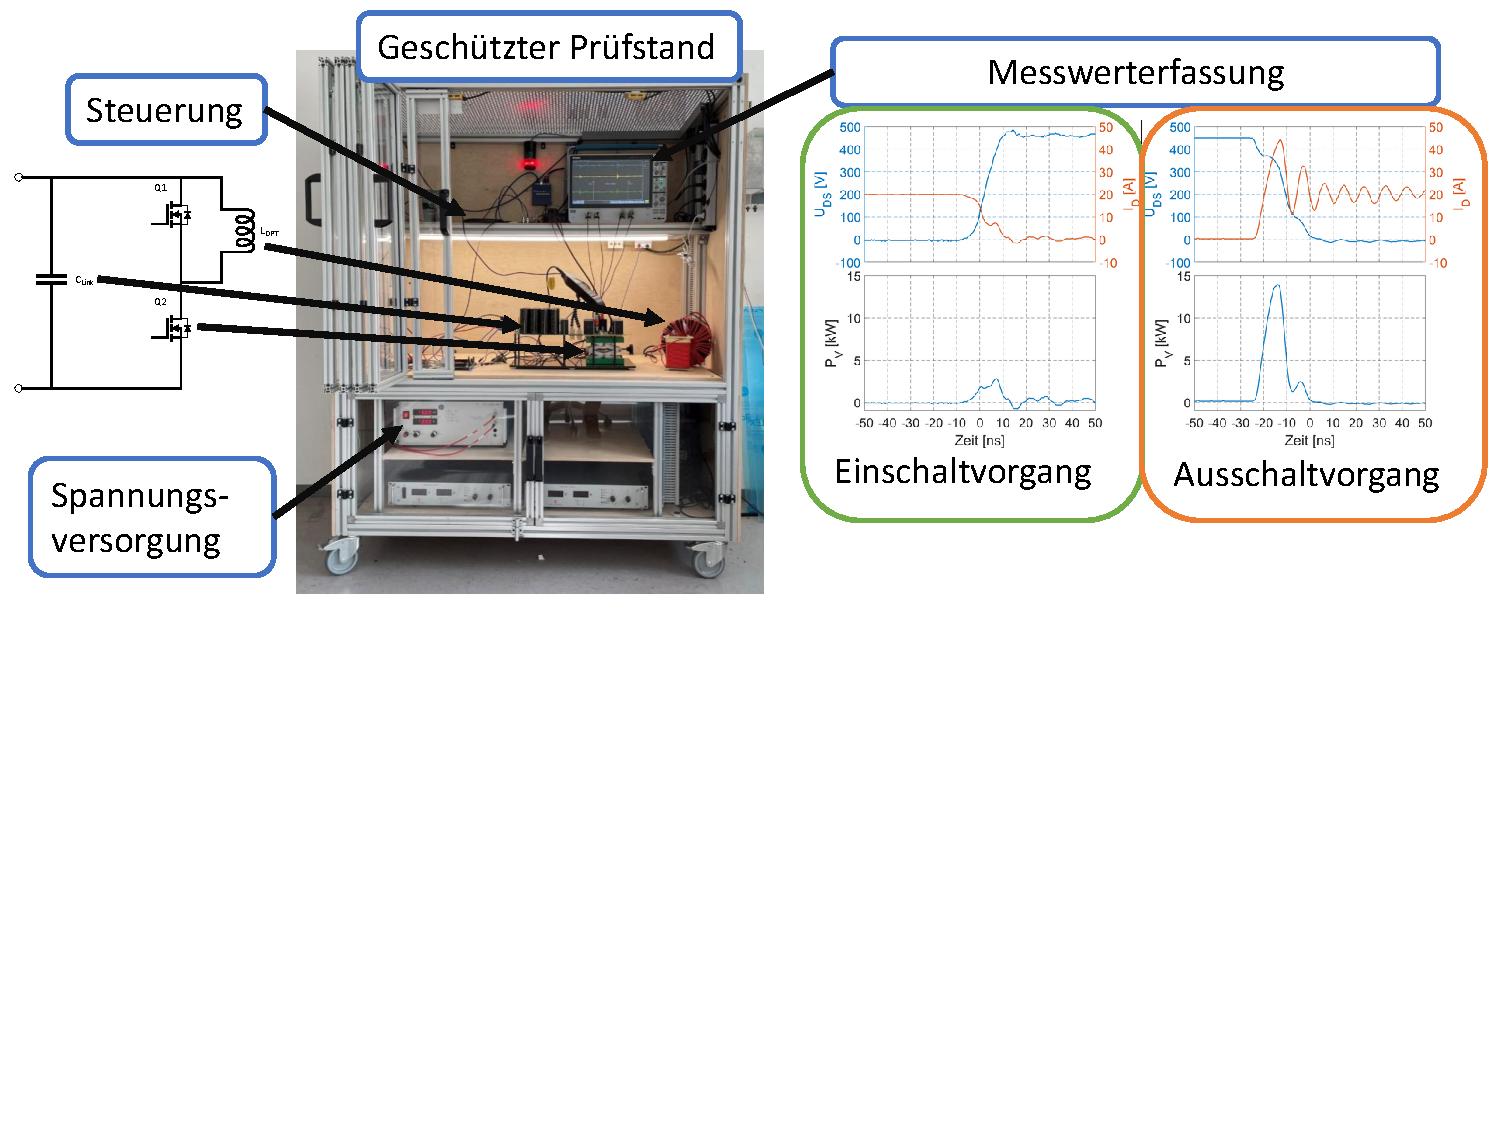
\includegraphics[width=0.95\linewidth]{content/Grafiken/DPT}
	\caption{Doppelpulstestprüfstand}
	\label{fig:dpt}
\end{figure}
Ein weiterer Punkt ist der direkte Blitzeinschlag in das Stromnetz, der zu einer Spannungserhöhung führt. Entsprechende Funktionen und Spannungsgeneratoren können in die Simulation eingebaut werden, um die auftretenden Überspannungen an den Halbleitern zu ermitteln. Bei der Betrachtung fällt auf, dass bei beiden Topologien aufgrund des Aufbaus immer ein leitender Pfad über die Dioden gewährleistet ist. Die Energie kann somit im Zwischenkreiskondensator aufgenommen werden, wobei auf die Dimensionierung und die auftretenden Überspannungen an den Halbleitern zu achten ist. Der Strompfad über die Dioden in den Kondensator ist in Abbildung \ref{fig:iafsurge} dargestellt und ist identisch mit dem des \gls{B6PFC}.
\begin{figure}[H]
	\centering
	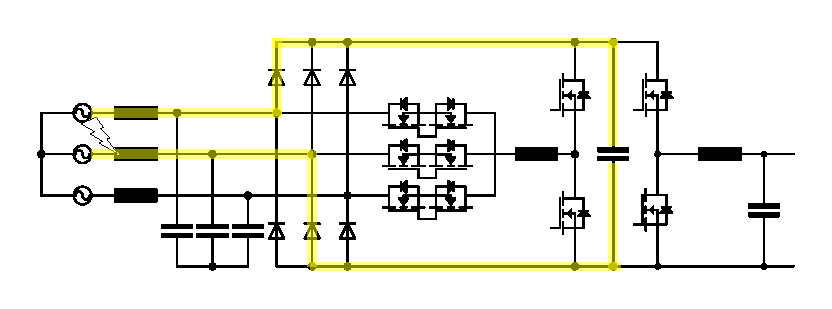
\includegraphics[width=0.95\linewidth]{content/Grafiken/IAF_surge}
	\caption{Strompfad im Fall eines Blitzeinschlags beim IAF}
	\label{fig:iafsurge}
\end{figure}
Die Schaltungen können außerdem durch Parallelbetrieb mit Interleaving am Ausgang oder bei entkoppelter Versorgung (durch getrennte Wicklungen am Netztransformator) als ausgangsseitige Reihenschaltung betrieben werden, um eine höhere Ausgangsspannung zu erzielen. Dabei sind weitere Regelungsparameter und Tests zur Betrachtung der Stabilität sowie des Auftretens unerwünschter Ausgleichsströme nötig. Um das Ziel einer Multimegawatt-Elektrolyseanlage zu erreichen, müssen mehrere Gleichrichter parallel betrieben werden. Daher ist die direkte Parallelisierung ein interessanter Aspekt für zukünftige Betrachtungen. Dies kann zunächst anhand von Simulationen durchgeführt werden, was den Rechenaufwand deutlich erhöht, um spätere Hardwaretests durchzuführen. Des weiteren kann der Hardwareaufbau in Kombination mit Echtzeitsystemen und Nachbildungen von Netz und Elektrolyseur durch Leistungsverstärker unter realen Bedingungen getestet werden. \\
